\documentclass[a4paper]{scrartcl}

\usepackage{amsmath}
\usepackage{amsfonts}
\usepackage{xspace}
\usepackage{xcolor}
\usepackage{tikz}
\usepackage{hyperref}
\hypersetup{
    colorlinks,
    linkcolor={red!50!black},
    citecolor={blue!50!black},
    urlcolor={blue!50!black}
}

\newcommand{\fort}{{\scshape{Fortran}}\xspace}
\newcommand{\mylanguage}{{\scshape{Fortress}}\xspace}
\title{Introduction to language theory and compiling\\
  Project -- Part 2}

  \author{Gilles {\scshape{Geeraerts}}\and Léonard {\scshape{Brice}} \and
  Sarah {\scshape{Winter}}}

\begin{document}

\maketitle


\begin{abstract}
This report gives an overview of the typical mistakes that were made, and explains the different choices you had for the implementation. It also aims to show you what a typical report should look like in terms of structure and how to explain your choices. Obviously, you are not supposed to give a list of potential mistakes in your report.
\end{abstract}

\section{Introduction}

The \mylanguage language is a simple imperative language which provides basic constructors: variable names, instructions to read and print them, \texttt{while} loops, comperators, etc. This second part of the project consisted in implementing a recursive-descent, LL(1) parser for \mylanguage.

\section{Preprocessing}

You first had to modify the grammar so as to make it LL(1):

\subsection{Removal of unproductive and/or unreachable variables}

There were no unproductive nor unreachable variables, but to prove it you had to execute the algorithm given in the course.

\subsection{Disambiguise the grammar}

\paragraph{Precedence}
The case of arithmetic expressions is practically the same as the one seen during the practicals. The novelty lies in the unary minus, which enjoys highest precedence. Adding the derivation <A> $\rightarrow$ MINUS <A> (where <A> denotes your most atomic terminal in <ExprArith>) implements this, because it ensures that the unary minus is ``glued'' to its corresponding expression.

% To handle the case of boolean expressions, note that the precedence rules of (NOT, AND, OR) are the same as (one could say ``isomorphic'') the ones of (UMINUS, TIMES, PLUS). In other words, NOT can be seen as a unary minus, AND as a multiplicative operator and OR as an additive one. This is consistent with the similarity of structure between $(\mathbb{B}, \wedge, \vee)$ (where $\wedge$ is conjunction and $\vee$ is disjunction) and $(\mathbb{N}, \times, +)$.

\paragraph{Left-factoring}
Here, you could blindly apply the algorithms provided during the lessons. You could however be slightly smarter regarding the ``else'': here, the grammar can be both left- and right-factored, which translates into adding a \texttt{MaybeElse} non-terminal.

\medskip

All the above modifications are implemented in the \verb#Fortress_Grammar.txt# file in the \verb#more/# directory.

\subsection{First, Follow and the action table}

The First and Follow sets, as well as the action table, can be computed by using the command \verb#java -jar dist/ProcessGrammar.jar -pat more/Fortress_Grammar.txt# (\texttt{pat} stands for ``print action table''). You can also write it to \texttt{filename.txt} by calling \verb#java -jar dist/ProcessGrammar.jar -wat filename.txt more/Fortress_Grammar.txt#

Please note that the algorithm provided to compute the First and Follow sets, as well as the action table, may not be completely correct. So, if you want to use it to generate an action table for your own grammar treat the result with caution. 

\section{A few words about the implementation}

\subsection{Grammar processing}

We implemented a simple grammar parser using \texttt{JFlex} (the language is simple enough to avoid using more complex tools). The First, Follow and Action Table computation, as well as their printing, are implemented in the \texttt{Grammar.java} class. Such implementation is meant to be as close as possible to the algorithm described in the Practical Session 6. The corresponding executable is implemented in the \texttt{ProcessGrammar.java} class.
Again, we do not guarentee that this implementation is error free.

Note that the \texttt{Pair.java} is simply a quick implementation of the pair type, to be able to \texttt{Map} pairs to something (instead of doing a \texttt{Map} of \texttt{Map}s).

\subsection{Modification of the \texttt{Symbol} class}

To get more flexibility about the manipulation of terminals and variables, we chose to heavily modify the \texttt{Symbol} class, and split it into several classes: the \texttt{Terminal} and \texttt{NonTerminal} classes, which are simply enums of (non-)terminals, the \texttt{Symbol} class which is the union of \texttt{Terminal} and \texttt{NonTerminal}, and the \texttt{Token} class which plays the role of the old \texttt{Symbol} class. \texttt{NonTerminal} and \texttt{Token} are unioned under the \texttt{TreeLabel} class, which represents labels of parse tree nodes (cf the \texttt{ParseTree} class). Please note that this is certainly not the best way to do it in terms of code quality.

\subsection{Computation of the parse tree}

The parser keeps track of the current token --- by current we mean here the one that is right after the reading head: the parser will never have to look at the token currently pointed by the reading head. It can look at it (this is the meaning of the \texttt{switch(current.getType())} construct), and can advance the reading head using the \texttt{match(term)} function, which checks that the current token is indeed the expected terminal, consumes it and moves to the next token (this is exactly the Match operation seen in class).

The parse tree is computed during the parsing. It is represented using the \texttt{ParseTree} class, which represents a tree as a root label and the list of its children which are themselves parse trees. This corresponds to the classical, recursive definition of labeled trees.

Thus, there is one function per non-terminal of the grammar, and each function returns the parse tree rooted in the corresponding non-terminal. For instance, assume the parser has input \texttt{READ(num)} and is currently calling \texttt{read()} (we omit the calls to \texttt{program()} etc for clarity). Then, the \texttt{read()} function will return the tree depicted in Figure~\ref{fig:readTree}

\begin{figure}[ht]
 \centering
 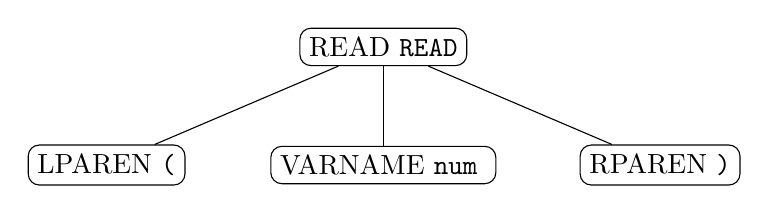
\begin{tikzpicture}[sibling distance=10em,
  every node/.style = {shape=rectangle, rounded corners,
    draw, align=center}]
  \node {READ \texttt{READ}}
    child { node {LPAREN \texttt{(}} }
    child { node {VARNAME \texttt{num} } }
    child { node {RPAREN \texttt{)}} };
\end{tikzpicture}
\caption{The output of \texttt{read()} on input \texttt{READ(num)}}
\label{fig:readTree}
\end{figure}

When there are more than one possible rule to apply, the parser looks at the next token (\texttt{switch(current.getType())}) and decides accordingly.

At the end of the parsing, the program has built the entire parse tree, and the \texttt{main} function (in \texttt{WriteTree.java}) outputs it to the \texttt{.tex} file given as argument.

Note that our parser does not output the numbers of the rules during the parsing. This is because you won't need them for Part 3, and it should be quite straightforward to add this feature anyway: we wrote the corresponding rule as a comment everytime (e.g. \texttt{// Program -> BEGIN PROGNAME Code END} at l.42 of \texttt{Parser.java}), so just add \texttt{System.out.println(number of the rule)}.

\subsection{Parsing errors}

Parsing errors are implemented in the \texttt{ParseException} class. It outputs the read token, the token it expected, and, when useful, a list of tokens it would have expected. Such tokens are simply the ones which have a non-empty cell in the action table in the corresponding non-terminal line. If the error happens while trying to parse a non-terminal (and not during a match), it additionally outputs the corresponding non-terminal.

\section{Conclusion}

The implementation we provide is not meant to be perfect. However, it should suffice for Part 3 if you did not manage to implement a working parser during Part 2.

\end{document}

%%% Local Variables: 
%%% mode: latex 
%%% TeX-engine: luatex
%%% TeX-master: t 
%%% TeX-command-extra-options: "-shell-escape"
%%% End:
